
\section{GPU Architecture}
GPUs (Graphical Processing Units) were originally created for 3D computer graphics. As GPUs have become more powerful and flexible, their usefulness for other computationally expensive tasks has become apparent. GPUs utilize massive amounts of parallelisation. Unlike multithreaded CPUs, the threads of GPUs work in a SIMD (Single Instruction, Multiple Data) fashion. A collection of threads, usually referred to as a warp or wavefront, run the same instructions on different data in parallel. Typically, one SIMD unit is responsible for multiple warps in order to interleave instructions to limit memory stalls, similar to hyper-threading on CPUs. This means that great care has to be taken when programming GPUs to utilise the threads optimally.\\

\begin{figure}[h]
    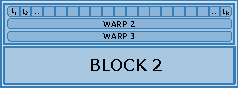
\includegraphics[scale=2]{figures/gpu_threads.pdf}
    \centering
    \caption{GPU thread hierarchy. A block consists of a number warps, all of which has a fixed number of threads (32 on modern NVIDIA hardware \citep{nvidiaadaarch}), besides the last which might have fewer.}
\end{figure}

CUDA (Compute Unified Device Architecture) has been the dominant programming model for utilising GPUs for general-purpose computations. CUDA allow kernels to be written in C++. Kernels refer to GPU programs that run in parallel. Kernels have limited options for synchronising between threads during execution. Therefore, algorithms typically consist of multiple kernels being dispatched from the CPU. To write high-performance kernels, a few factors have to be kept in mind. Note that we specifically refer to the architecture of modern NVIDIA GPUs, however, similar concepts hold true for other architectures.

\subsection{Thread Occupancy}
Thread occupancy refers to the percentage of the maximum possible warps being active at any given time. On NVIDIA GPUs, occupancy is typically measured per SM (Streaming Multiprocessor). Each SM can execute a limited amount of blocks and warps concurrently. If a subset of warps within a block takes longer to complete than the rest, it prevents new blocks from launching. Similarly, if a subset of blocks takes longer than the rest, it blocks the kernel from finishing. Besides leaving cores unused, it also makes the running cores less efficient as SIMD units have fewer warps to interleave. It is therefore crucial to balance work across warps and blocks \citep{Jeon2022}.

\subsection{Memory Access}
Memory access patterns can have a large impact on the performance of kernels. Because warps execute in a SIMD fashion, whenever data is accessed, the whole warp has to wait until the data has been fetched for all threads. It is therefore beneficial for warps to fetch data consecutive in memory. Because the L1 cache is local to each SM, it is also beneficial for threads within a block to access data close in memory.\\

Modern GPUs are prone to memory bandwidth bottlenecks. This means that situations occur where all warps managed by a SIMD unit are stalled because of memory reads. For this reason, it can at times be beneficial to use techniques such as \textit{recomputation} and \textit{kernel fusion}. \textit{Recomputation} attempts to lower the amount of memory accessed by recomputing results instead of fetching them from memory. This shifts more load to the ALU (Arithmetic Logic Unit), which may otherwise be idle. \textit{Kernel fusion} attempts the same by avoiding loads and stores by merging consecutive kernels and keeping the data in registers.

\begin{figure}[h]
    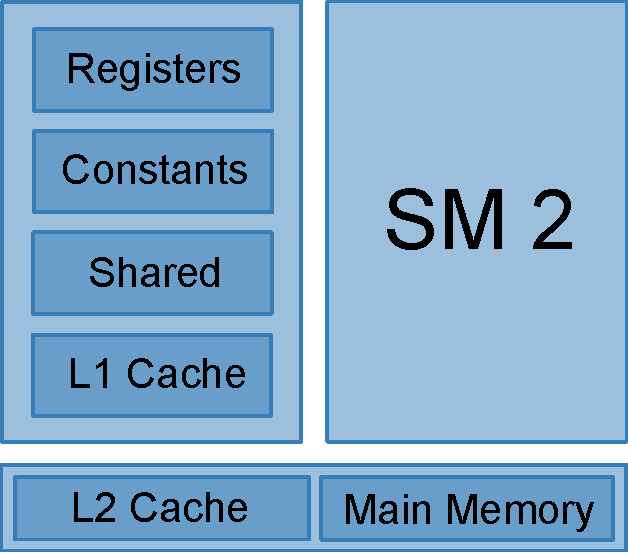
\includegraphics[scale=0.5]{figures/gpu_memory.pdf}
    \centering
    \caption{GPU memory hierarchy. SMs share registers, constants, shared memory and L1 cache, whereas L2 cache and memory is shared between SMs. Generally, memory is accessed fastest in registers and slowest in main memory \citep{nvidiaadaarch}.}
    \label{gpu_memory}
\end{figure}

As illustrated in Figure \ref{gpu_memory}, registers are shared between all warps in a SM unit. This means that the amount of registers used by a kernel can limit the amount of warps that can run in parallel.

\subsection{Divergence}
Because all threads of a warp execute in lockstep, branching can lead to performance problems if the threads diverge. If a branch is taken by a subset of threads in a warp, the whole warp waits until those threads are done executing the branch. It is therefore beneficial to assign work to threads such that all threads of a warp take similar branches.

\subsection{Floating Point Formats}\label{float_speed}
Modern GPU architectures are optimized for 32-bit and 16-bit floats. NVIDIA report 64 times fewer 64-bit float FLOPS (Floating Point Operations Per Second) compared to 32-bit floats on their ADA architecture \citep{nvidiaadaarch}.
It is therefore advantageous to do as many operations as possible with 32-bit floats.
